\documentclass[border=10pt]{standalone}
\usepackage{pgfplots}
\pgfplotsset{compat=1.18}
\usepgfplotslibrary{colormaps}

\begin{document}
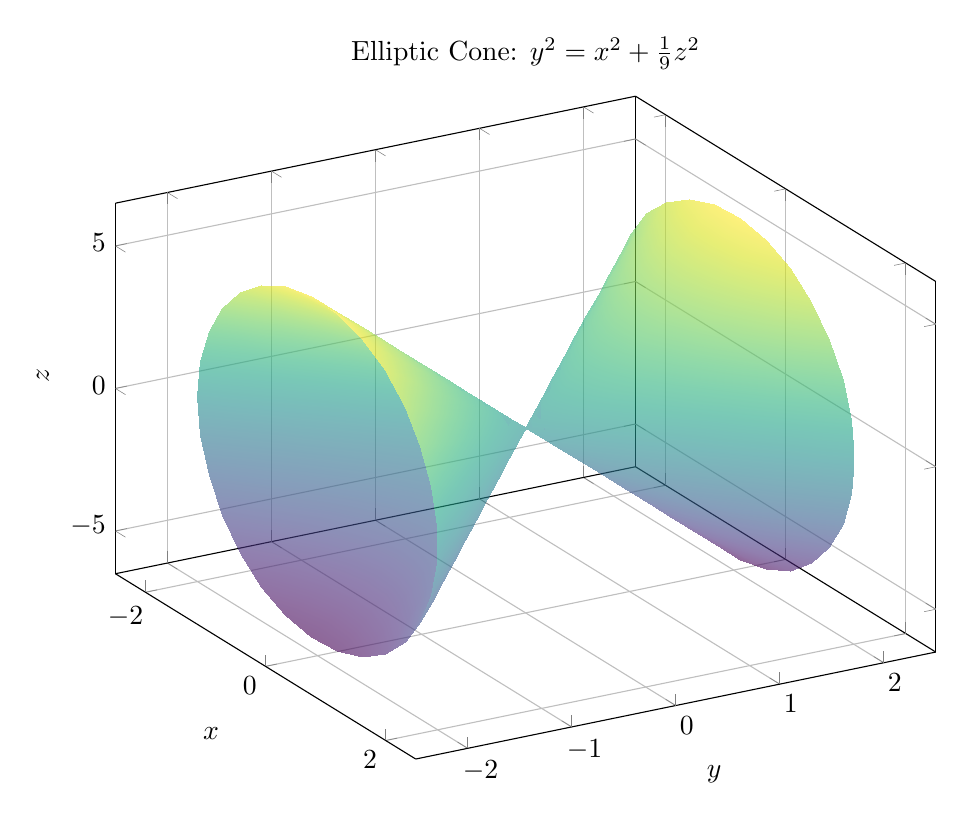
\begin{tikzpicture}
\begin{axis}[
    view={60}{30},
    xlabel={$x$},
    ylabel={$y$},
    zlabel={$z$},
    title={Elliptic Cone: $y^2 = x^2 + \frac{1}{9}z^2$},
    domain=0:360,
    y domain=-2:2,
    samples=30,
    samples y=20,
    colormap/viridis,
    grid=major,
    width=12cm,
    height=10cm,
    zmin=-6.5,
    zmax=6.5,
    xmin=-2.5,
    xmax=2.5,
    ymin=-2.5,
    ymax=2.5,
]
% Parameterization: x = v*cos(u), y = v, z = 3*v*sin(u)
\addplot3[surf, opacity=0.6, shader=interp] ({y*cos(x)}, {y}, {3*y*sin(x)});
\end{axis}
\end{tikzpicture}
\end{document}